\documentclass[12pt]{article}
\usepackage[margin=1in]{geometry}
\usepackage[all]{xy}

\usepackage{amsmath,amsthm,amssymb,color,latexsym,soul}
\usepackage{geometry}        
\geometry{letterpaper}    
\usepackage{graphicx}
\usepackage{enumitem}
\usepackage{listings}
\usepackage{xcolor}
\usepackage{bm}

\definecolor{codegreen}{rgb}{0,0.6,0}
\definecolor{codegray}{rgb}{0.5,0.5,0.5}
\definecolor{codepurple}{rgb}{0.58,0,0.82}
\definecolor{backcolour}{rgb}{0.95,0.95,0.92}

\lstdefinestyle{mystyle}{ % taken from: https://www.overleaf.com/learn/latex/Code_listing
    backgroundcolor=\color{backcolour},   
    commentstyle=\color{codegreen},
    keywordstyle=\color{magenta},
    numberstyle=\tiny\color{codegray},
    stringstyle=\color{codepurple},
    basicstyle=\ttfamily\footnotesize,
    % breakatwhitespace=false,         
    breaklines=true,                 
    captionpos=b,                    
    keepspaces=true,                 
    % numbers=left,                    
    numbersep=5pt,                  
    % showspaces=false,                
    % showstringspaces=false,
    % showtabs=false,                  
    % tabsize=2
}

\lstset{style=mystyle}

\newtheorem{task}{Task}
\newenvironment{solution}[1][\it{Solution}]{\textbf{#1. } }{$\square$}
\newtheorem{subtask}{\; \; \it{Part}}


\begin{document}
\noindent Asaad Mohammedsaleh \hfill CS249 Assignment 2\\
KAUST Spring 2025 \hfill Genome Assembly and Evaluation


\hrulefill


\section{Task 1.1}

\section{Task 1.2}

\section{Task 1.3}

\subsection{Task 1.3.1}

\begin{figure}[h]
    \centering
    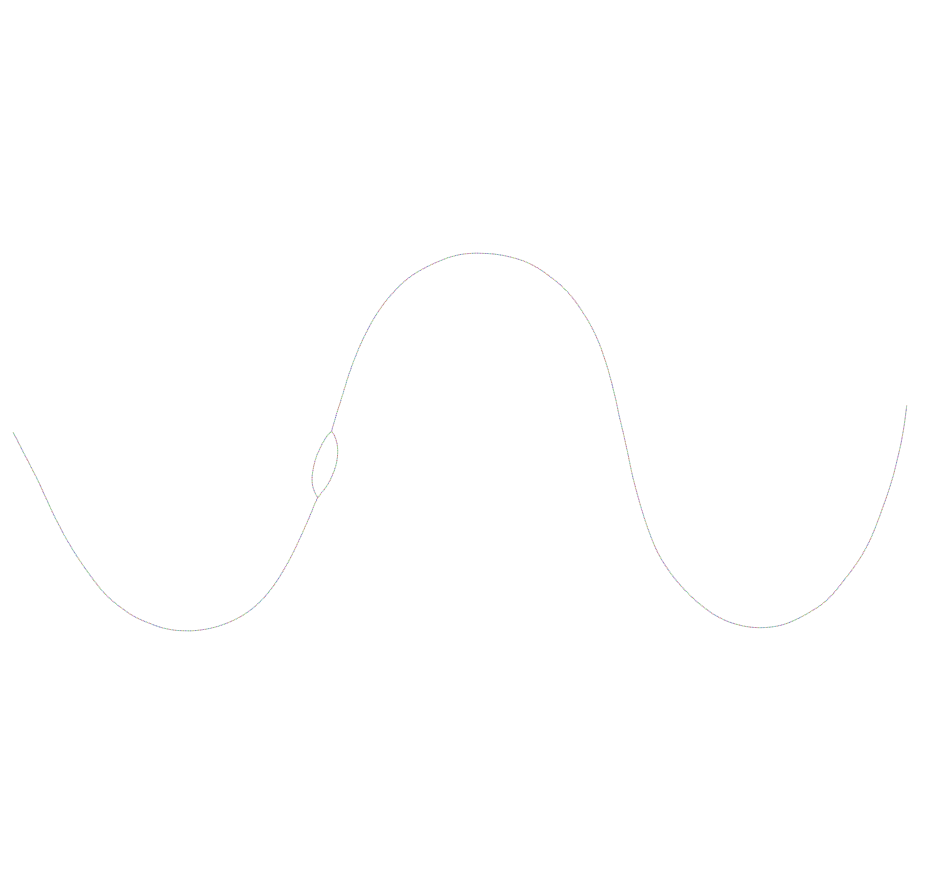
\includegraphics[width=0.5\textwidth]{../toy_dataset/reads_b_k_40.png}
    \caption{Bandage visualization of DBG for k=40}
\end{figure} 

\subsection{Task 1.3.2}

\begin{figure}[h]
    \centering
    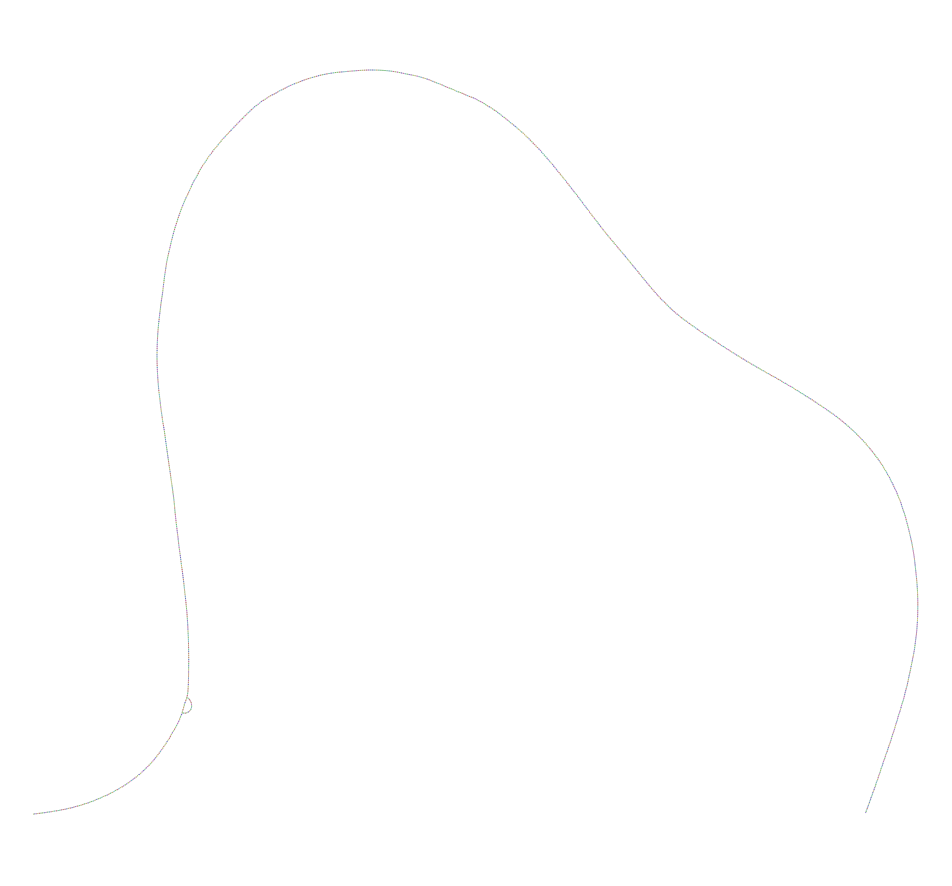
\includegraphics[width=0.5\textwidth]{../toy_dataset/r-k-35.png}
    \caption{Bandage visualization of DBG contigs for k=35 on reads\_r.fastq}
\end{figure} 

\begin{figure}[h]
    \centering
    
\includegraphics[width=0.5\textwidth]{../toy_dataset/r-k-45.png}
    \caption{Bandage visualization of DBG contigs for k=45 on reads\_r.fastq}
\end{figure} 



\subsection{Task 1.3.3}

\subsection{Task 1.3.4}




\end{document}
